
\begin{table}[H]
    \centering
    \hspace*{-1.75cm}
    \begin{tabular}{rc|c|>{\centering\arraybackslash}p{0.5\linewidth}|} 
        \cline{3-4} 
        & Fallabbildung & Bedingungen & Bewertung \\\cline{3-4}
        \vspace{-1.35em} \\ \cline{3-4}
            1 & \begin{minipage}{0.25\textwidth}
                    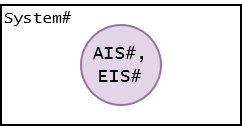
\includegraphics[width=\linewidth]{gfx/IA41.drawio.png} 
                \end{minipage}
                &$\begin{array}{l}
                    \scriptstyle EIS\# \;=\; AIS\#; \\
                    \scriptstyle EIS\# \;\subset\; System\# \\
                  \end{array}$ 
                &\begin{minipage}{0.5\textwidth} 
                    \smaller
                    \textit{Optimales Ergebnis}: Geschätzter Impact stimmt mit \acsfont{AIS\#} überein. Spricht für eine sehr hilfreiche \ac{IA}.
                \end{minipage} 
            \\ \cline{3-4}
            2 & \begin{minipage}{0.25\textwidth}
                    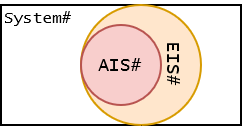
\includegraphics[width=\linewidth]{gfx/IA42.drawio.png} 
                \end{minipage}
                &$\begin{array}{l}
                    \scriptstyle |EIS\#| \;>\; |AIS\#|; \\
                    \scriptstyle AIS\# \;\subset\; EIS\#; \\
                    \scriptstyle EIS\# \;\subseteq\; System\# \\
                  \end{array}$ 
                & \begin{minipage}{0.5\textwidth} 
                    \smaller
                    \textit{Gutes sicheres Ergebnis}: Alle eingetroffenen Änderungen wurden richtig eingeschätzt und die Differenz der Mengen ist nicht sehr groß.
                \end{minipage} 
            \\ \cline{3-4}
            3 & \begin{minipage}{0.25\textwidth}
                    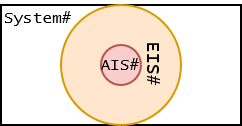
\includegraphics[width=\linewidth]{gfx/IA43.drawio.png} 
                \end{minipage}
                &$\begin{array}{l}
                    \scriptstyle |EIS\#| \;\gg\; |AIS\#|; \\
                    \scriptstyle AIS\# \;\subset\; EIS\#; \\
                    \scriptstyle EIS\# \;\subseteq\; System\# \\
                  \end{array}$ 
                & \begin{minipage}{0.5\textwidth}
                    \smaller
                    \textit{Schwaches sicheres Ergebnis}: Alle Änderungen wurden richtig eingeschätzt, jedoch ist die Differenz der Mengen sehr groß und es wurde viele weitere Entitäten falsch markiert.
                \end{minipage} 
            \\ \cline{3-4}
            4 & \begin{minipage}{0.25\textwidth}
                    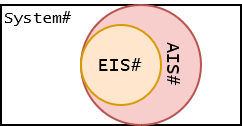
\includegraphics[width=\linewidth]{gfx/IA44.drawio.png} 
                \end{minipage}
                &$\begin{array}{l}
                    \scriptstyle |AIS\#| \;>\; |EIS\#|; \\
                    \scriptstyle EIS\# \;\subset\; AIS\#; \\
                    \scriptstyle AIS\# \;\subseteq\; System\# \\
                  \end{array}$ 
                & \begin{minipage}{0.5\textwidth}
                    \smaller
                    \textit{Unsicheres Ergebnis}: Die Abschätzung verfehlt die komplette Abdeckung aller betroffenen Änderungen.
                \end{minipage} 
            \\ \cline{3-4}
            5 & \begin{minipage}{0.25\textwidth}
                    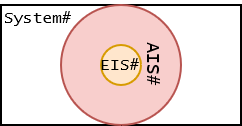
\includegraphics[width=\linewidth]{gfx/IA45.drawio.png} 
                \end{minipage}
                &$\begin{array}{l}
                    \scriptstyle |AIS\#| \;\gg\; |EIS\#|; \\
                    \scriptstyle EIS\# \;\subset\; AIS\#; \\
                    \scriptstyle AIS\# \;\subseteq\; System\# \\
                  \end{array}$ 
                & \begin{minipage}{0.5\textwidth}
                    \smaller
                    \textit{Stark unsicheres Ergebnis}: Die Abschätzung verfehlt die betroffenen Änderungen sehr. Die große Diskrepanz bedarf weiterer Arbeit zum Erschließen der \acsfont{AIS\#}.
                \end{minipage} 
            \\ \cline{3-4}
            6 & \begin{minipage}{0.25\textwidth}
                    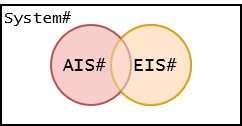
\includegraphics[width=\linewidth]{gfx/IA46.drawio.png} 
                \end{minipage}
                &$\begin{array}{l}
                    \scriptstyle |AIS\# \;\cap\; EIS\#|\; > \; 0; \\
                    \scriptstyle EIS\# \;\neq\; AIS\#; \\
                    \scriptstyle EIS\# \;\subseteq\; System\# \\
                  \end{array}$ 
                & \begin{minipage}{0.5\textwidth}
                    \smaller
                    \textit{Verfehltes Ergebnis}: Die Abschätzung verfehlt die komplette Abdeckung aller betroffenen Änderungen und beinhaltet nicht betroffene Entitäten.
                \end{minipage} 
            \\ \cline{3-4}
            7 & \begin{minipage}{0.25\textwidth}
                    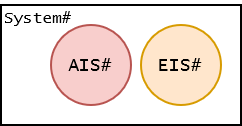
\includegraphics[width=\linewidth]{gfx/IA47.drawio.png} 
                \end{minipage}
                &$\begin{array}{l}
                    \scriptstyle |AIS\# \;\cap\; EIS\#|\; = \; 0; \\
                    \scriptstyle EIS\# \;\subset\; System\#; \\
                  \end{array}$ 
                & \begin{minipage}{0.5\textwidth}
                    \smaller
                    \textit{Stark verfehltes Ergebnis}: Extremere Version von Fall 6.
                \end{minipage} 
            \\ \cline{3-4}
        \cline{3-4}
    \end{tabular}
    \caption{Mögliche \acsfont{AIS\#}/\acsfont{EIS\#} Abhängigkeiten nach Arnold et al. \cite[299]{app_bohner}}
    [Eigene Darstellungen]
    \label{tab:eis_ais}
\end{table}
